\documentclass[PROP_AGutteridge_CS.tex]{subfiles}

\begin{document}

\chapter{Related Work}
In order to provide context to where the proposed project will fit in with existing technologies, comparable systems will be reviewed and contrasted. 

\section{Web applications}
\subsection{GoPubMed}
Developed by Michael Schroeder and colleagues at Dresden University, GoPubMed is a server and web interface that provides PubMed search results informed by the Gene Ontology database\cite{doms}. By extracting terms present in the Gene Ontology database from abstracts, GoPubMed has an improved vocabulary for genes and the gene products, enabling discovery of relevant papers that may be missed by the default PubMed search algorithm. The web interface also has additional functionality by providing shortcuts to 'Highly Related Concepts', authors and locations (Fig.1a), as well as visual representations of the data (Fig.1b) \\

\begin{figure}
	\begin{subfigure}{1\textwidth}
		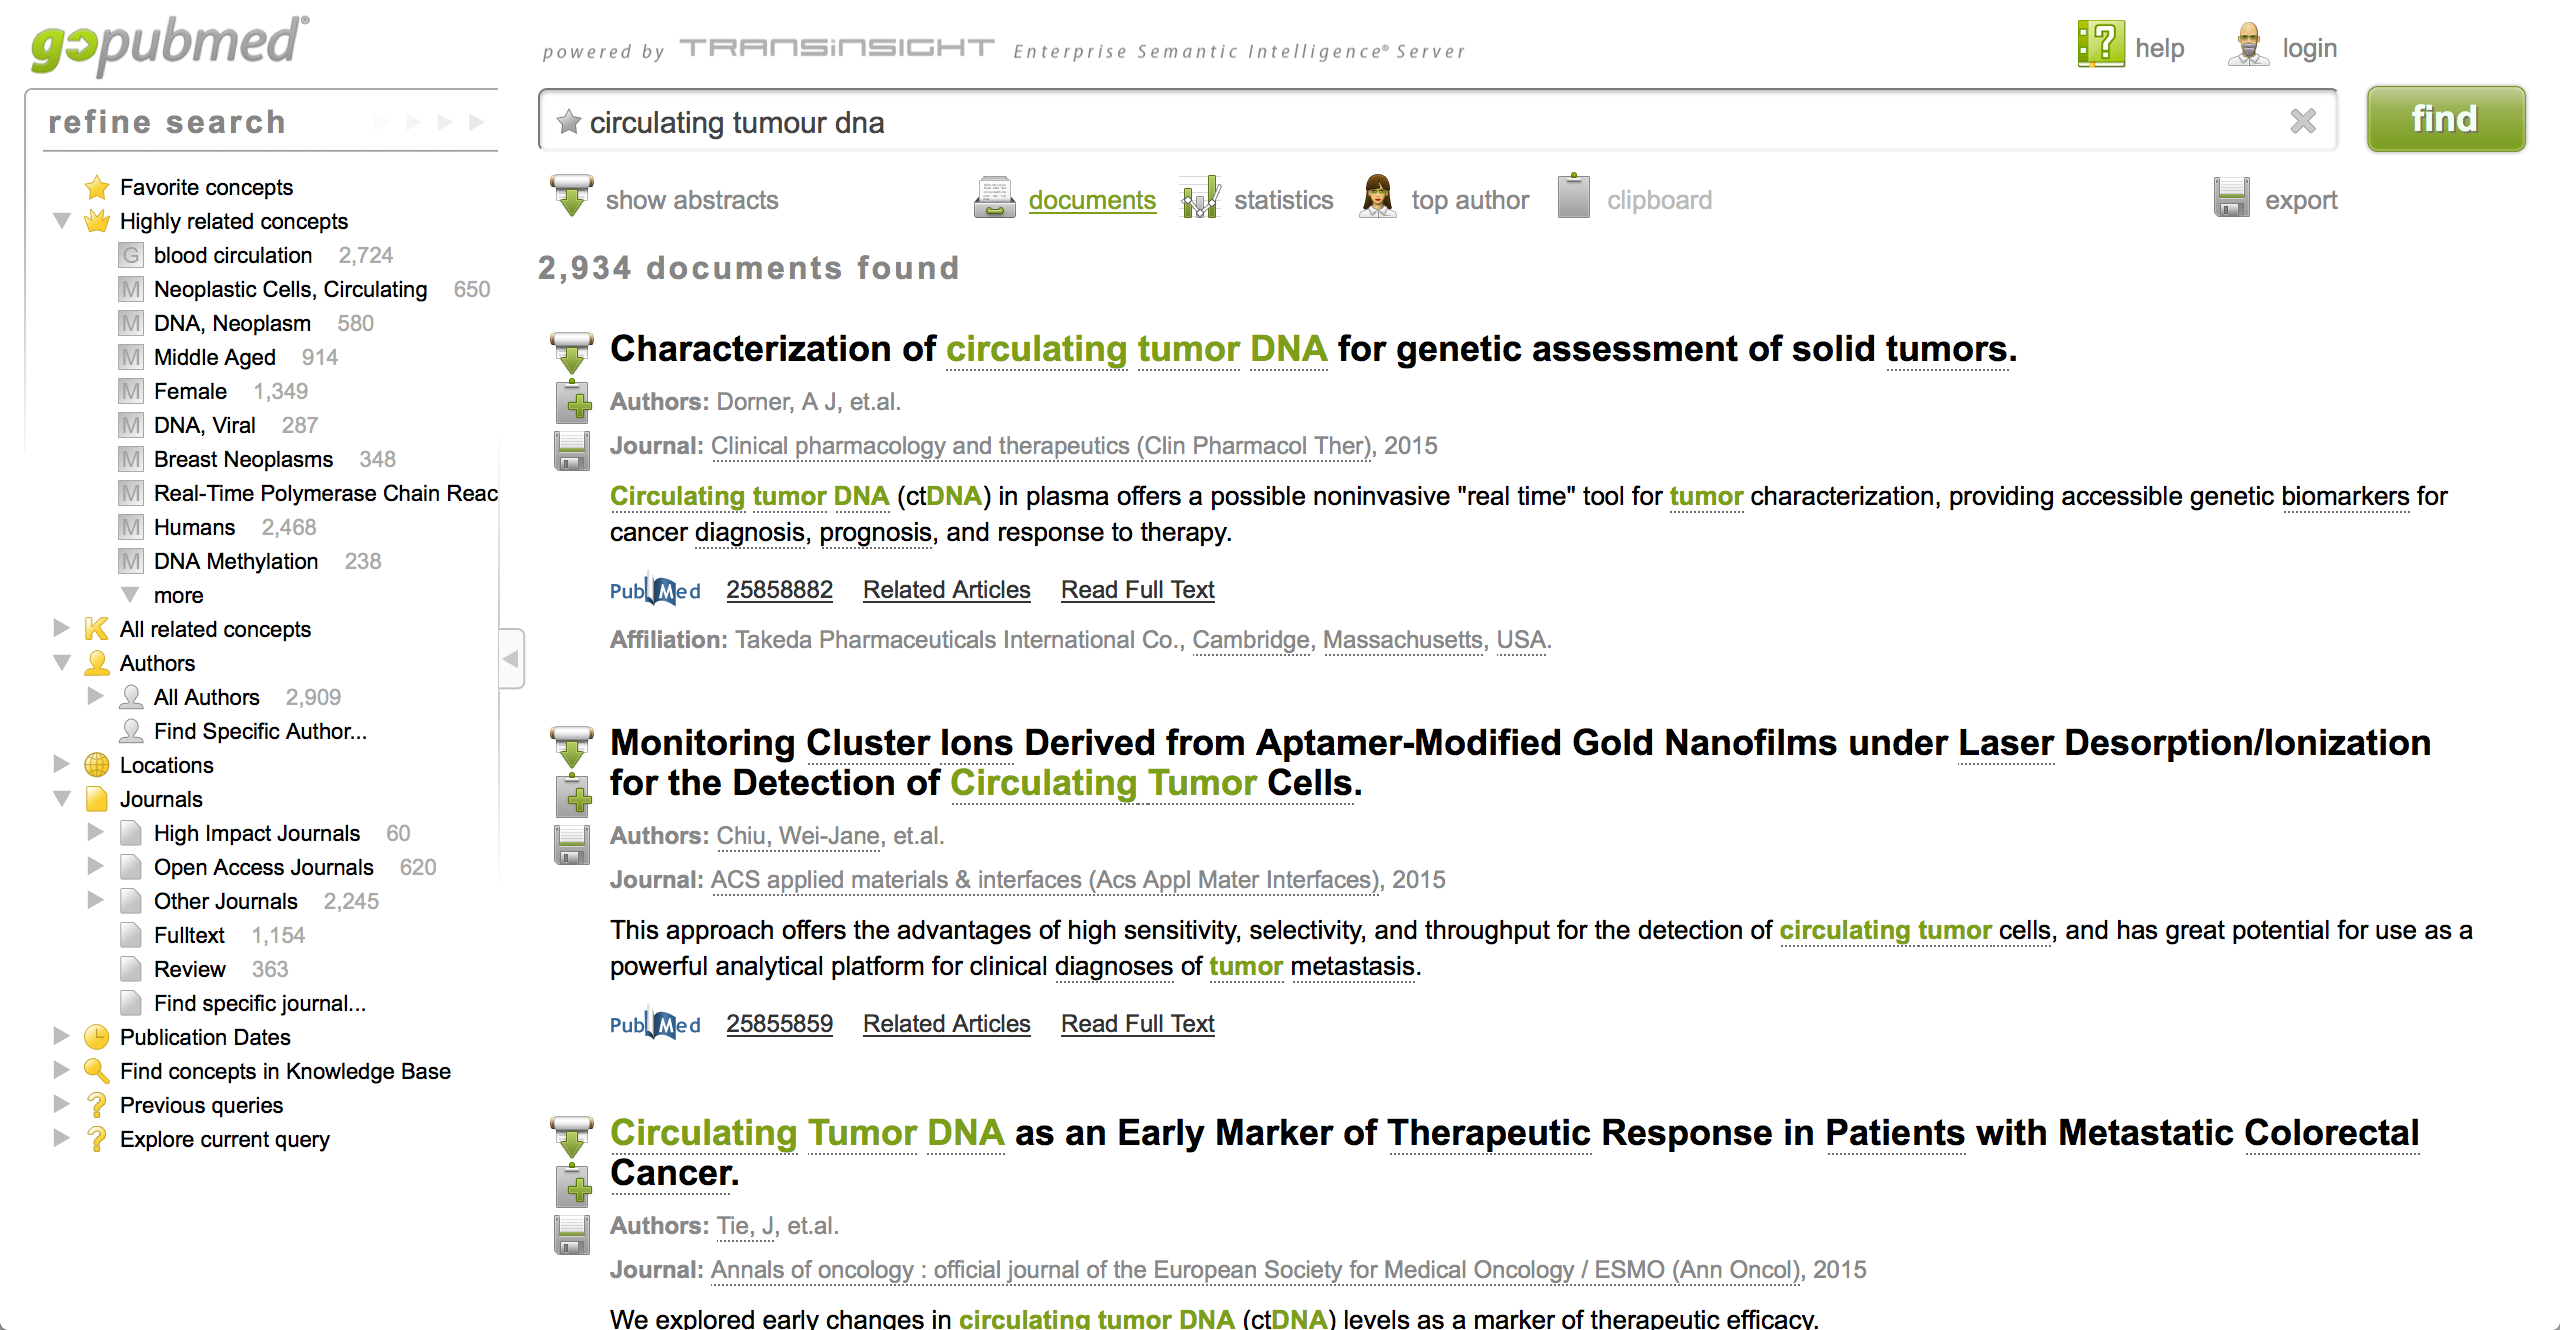
\includegraphics[width=\textwidth]{../lib/images/GPM1}
		\label{fig:GPM1}
		\subcaption{Documents view}
	\end{subfigure}\\
	\begin{subfigure}{1\textwidth}
		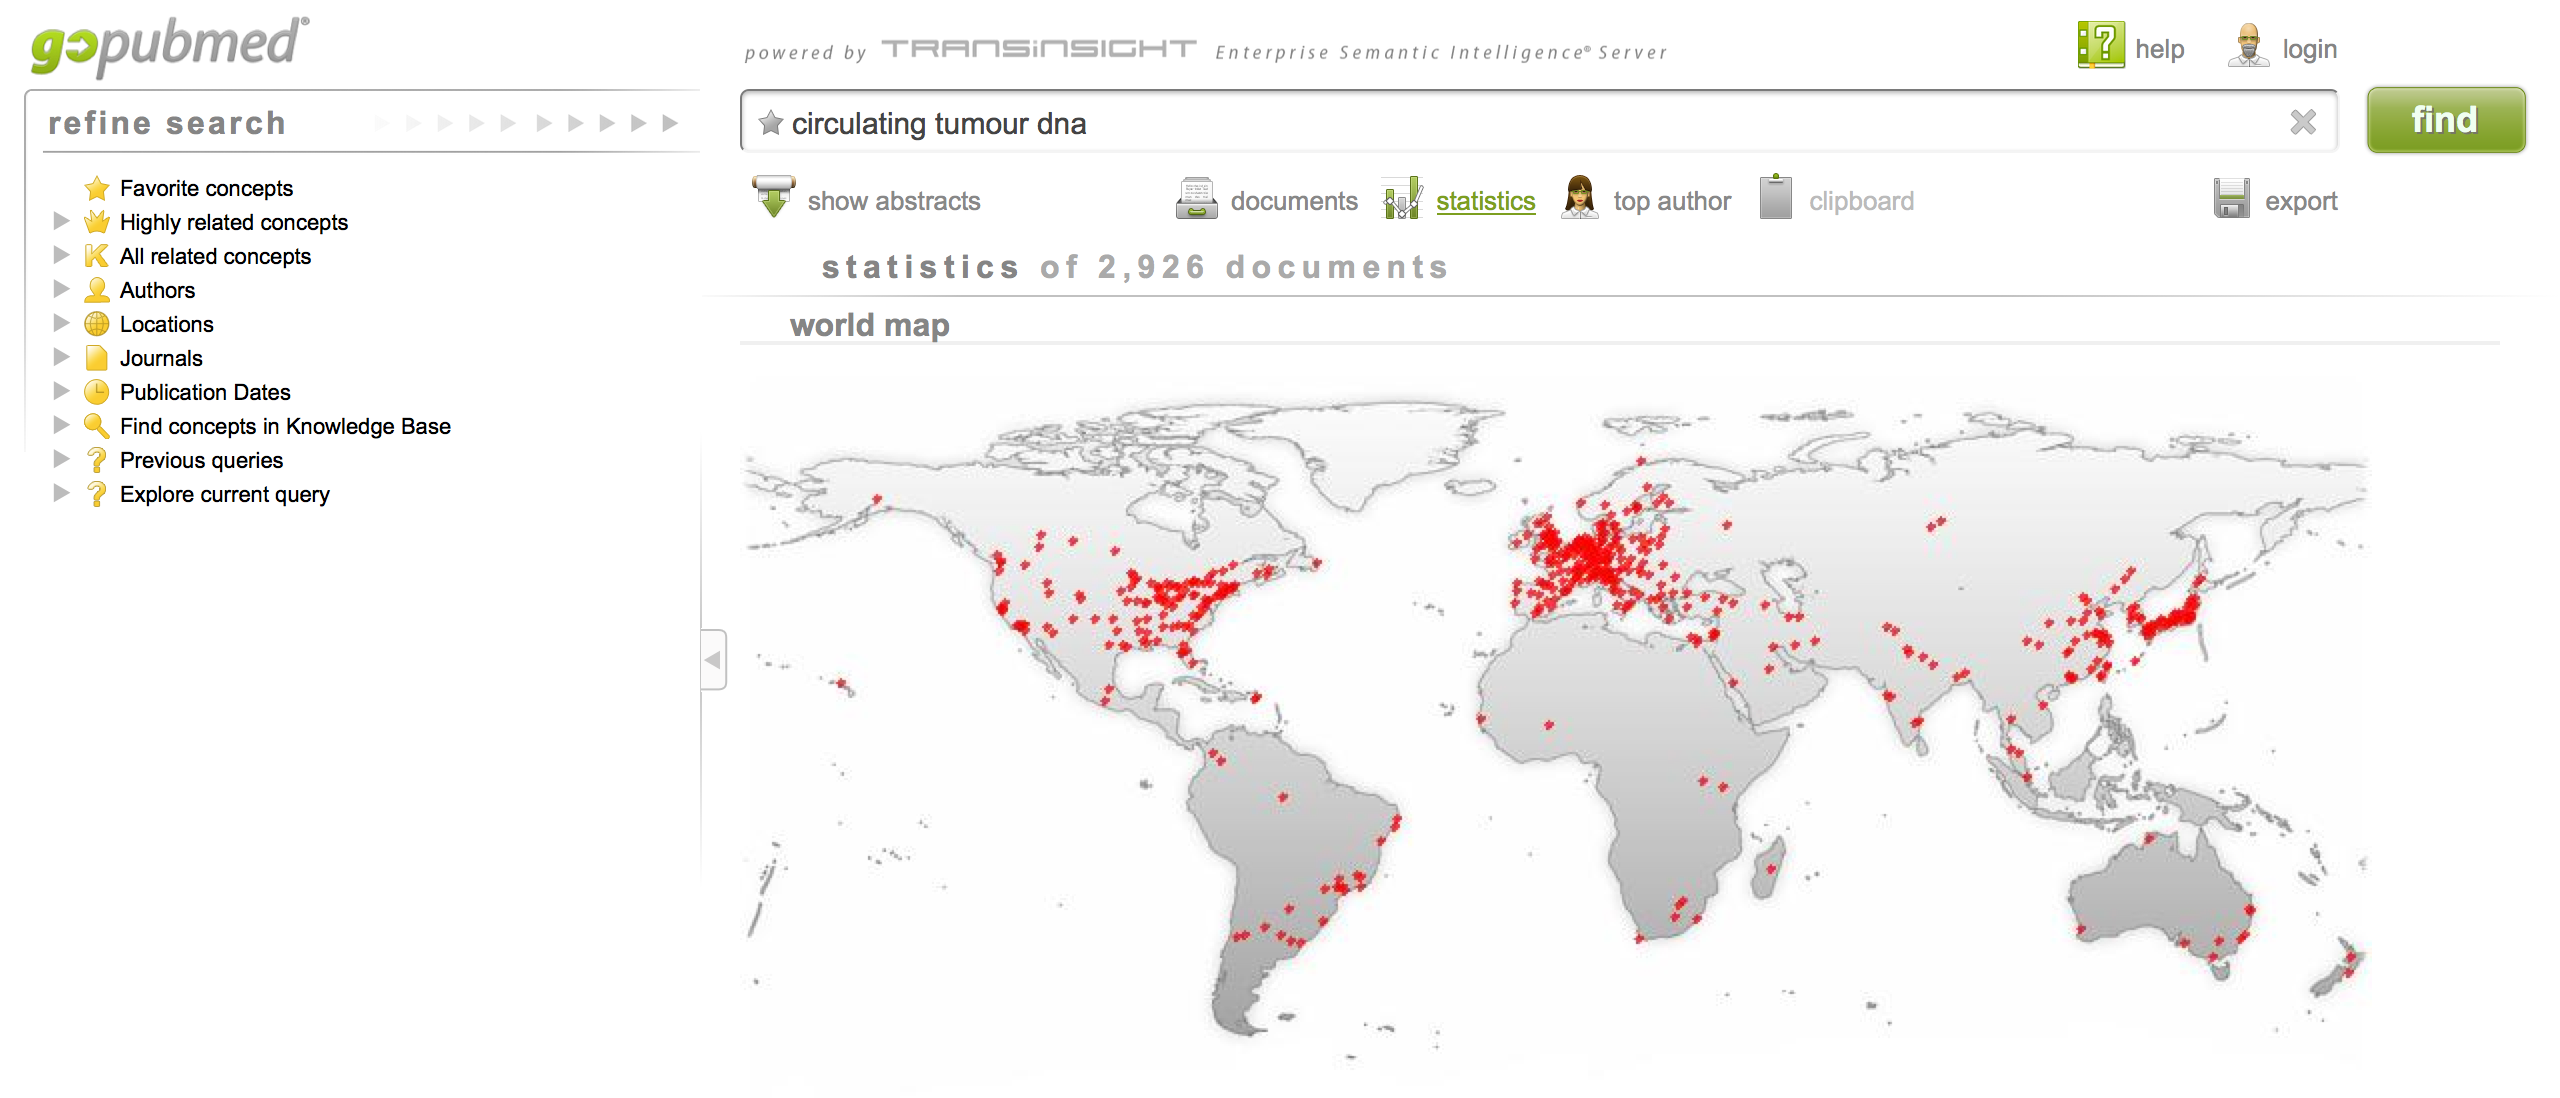
\includegraphics[width=\textwidth]{../lib/images/GPM4}
		\label{fig:GPM4}
		\subcaption{Statistics view}
	\end{subfigure} 
\caption{Web interface of GoPubMed. a) Screen after a search term has been entered. The main component of the page is the list of relevant documents, ordered by latest publication date. Additional filters are available in the sidebar to the right. b) When the 'statistics' hyperlink is followed, graphics are generated from the result data. This screenshot demonstrates a generated static JPEG showing the geographical locations of all authors.}
\end{figure}

\noindent GoPubMed presents users with a larger number of papers related to their topic of interest by retrieving papers with MeSH terms contained in their abstracts. Due to the aims of the project as described\cite{doms}, the applicability is largely limited to the field of Molecular Biology where genes and proteins are of primary interest. Mechanisms through which a large number of results can be refined are also provided as part of the interface, allowing the user to specify, for example, that only papers authored in the United Kingdom should be shown. Although a map of authors is generated (Fig.1b), it is static and therefore does not allow direct user interaction. % How much opinion should I include? e.g. I feel that there are too many filter categories of equal prominence, so potentially useful fields are a bit obscured to the user. 
Overall I feel like this website is achieving similar but not exactly what I want because it is less focused and still produces results as a textual list. I would prefer to do things dynamically as all information needed is already available in fields (don't intend to look in abstracts)

Talk about concepts that come up really high but really are not very helpful i.e. Middle-Aged, Male, Female !!

\subsection{HubMed}
kind of just another interface to pubmed but provides citations. deprecated? another figure.

\subsection{Microsoft Academic Map}
deprecated, high level information that often navigates away to new page (based on whether academic, institution is clicked on) resolution of institutions improves as map is zoomed = good! Unable to resolve UCL, potentially due to multiple locations?

\subsection{Conclusion?}
Combination of these with emphasis on visual interface, institution locations and entity separation, organisation of MeSH keywords. OBJECTIVES.

\end{document}